\documentclass{anstrans}

%% INCLUDING THE PREAMBLE
\usepackage[usenames,dvipsnames]{xcolor}
\usepackage{listings,amsmath}
\usepackage{microtype,todonotes}

%% CPATION SETUP
\usepackage{caption}
\usepackage{subcaption}
\captionsetup{belowskip=12pt,aboveskip=4pt}

\usepackage{fancyvrb}
\VerbatimFootnotes

%% HYPERLINKS
\usepackage[debug]{hyperref}

%% GRAPHICS RELATED
\usepackage{graphicx}
\usepackage[outdir=./tmp/]{epstopdf}
\graphicspath{{../images/}{./}{./tmp/}}
\DeclareGraphicsExtensions{.eps, .pdf, .jpeg, .png}

%% UNITS
\usepackage{siunitx}

%% USER COMMANDS
\newcommand{\iso}[2]{${}^{#2}${#1}}
\newcommand{\figurewidth}{0.45\textwidth}
\newcommand{\micron}{$\mu$m }

%%%%%%%%%%%%%%%%%%%%%%%%%%%%%%%%%%%%%%%%%%%%%%%%%%%%%%%%%%%%%%%%%%%%%%%%%%%
%                                                                         %
%                        AUTHOR, TITLE, and ABSTRACT                      %
%                                                                         %
%%%%%%%%%%%%%%%%%%%%%%%%%%%%%%%%%%%%%%%%%%%%%%%%%%%%%%%%%%%%%%%%%%%%%%%%%%%
\title{Simulated Energy Depostion in Thin Polymeric Films}
\author{Matthew J. Urffer, L. F. Miller \and A. Mabe}
\institute{
University of Tennessee, Knoxville, TN, 37916
}

\begin{document}
%%%%%%%%%%%%%%%%%%%%%%%%%%%%%%%%%%%%%%%%%%%%%%%%%%%%%%%%%%%%%%%%%%%%%%%%%%%
%                                                                         %
%                               INTRODUCTION                              %
%                                                                         %
%%%%%%%%%%%%%%%%%%%%%%%%%%%%%%%%%%%%%%%%%%%%%%%%%%%%%%%%%%%%%%%%%%%%%%%%%%%
\section{Introduction}
The Department of Homeland Security (DHS) continues to fund research for nuclear material detectors.
These detectors are designed to replace the \iso{He}{3} detectors currently installed as radiation portal monitors.
DHS / DNDO (along with PNNL) has determined a set of objectives that replacement technologies should meet, of which the effective discrimination between gammas (which can occur in medical isotopes) and neutrons (indicative of special nuclear material) is emphasized \cite{kouzes_neutron_2010,kouzes_neutron_1999}. 

A possible replacement technology being investigated is \iso{Li}{6} (thermal cross section of 940 barns) embedded in a scintillating polymer matrix.
Upon the absorption of a neutron \iso{Li}{6} fissions into two fragments; an alpha particle of energy 2.05 MeV and a triton of energy 2.73 MeV.
The Q-value of 4.78 MeV makes \iso{Li}{6} an attractive alternative compared to other reactions such as the \iso{He}{3} reaction which has a Q-value of 0.756 MeV or \iso{B}{10} (Q-value of 2.31 MeV).

%%%%%%%%%%%%%%%%%%%%%%%%%%%%%%%%%%%%%%%%%%%%%%%%%%%%%%%%%%%%%%%%%%%%%%%%%%%
%                                                                         %
%                                 THEORY                                  %
%                                                                         %
%%%%%%%%%%%%%%%%%%%%%%%%%%%%%%%%%%%%%%%%%%%%%%%%%%%%%%%%%%%%%%%%%%%%%%%%%%%
\section{Theory}
Neutron detectors often utilize a material doped with an isotope of large thermal cross section for absorption such as \iso{He}{3}, \iso{Li}{6} or \iso{B}{10}. 
When these materials absorb a neutron the nucleus of the isotope becomes unstable and fissions into reaction products.
These reaction products (having an initial kinetic energy equal to the Q-value of the neutron absorption reaction) travel through the material, transferring their kinetic energy to the material.
Photon interactions in the detector occur when a photon scatters off a single electron in a Compton scattering event and transfers a portion of its energy to the electron.
The Compton electron produces a cascade of secondary electrons in the material, which, depending upon the energy, may deposit a majority of its energy in the detector.
The difference in the energy deposition in the material from charged particles and from photon interactions introduces an opportunity to exploit the difference in energy deposition in order to maximize the discrimination between neutron and photon interactions in a detector.

%%%%%%%%%%%%%%%%%%%%%%%%%%%%%%%%%%%%%%%%%%%%%%%%%%%%%%%%%%%%%%%%%%%%%%%%%%%
%                                                                         %
%                       DESCRIPTION OF WORK                               %
%                                                                         %
%%%%%%%%%%%%%%%%%%%%%%%%%%%%%%%%%%%%%%%%%%%%%%%%%%%%%%%%%%%%%%%%%%%%%%%%%%%
\section{Description of Work}
The energy deposition of neutrons and gammas was investigated for polymeric films containing \iso{LiF}{6} of thickness ranging from \SI{15}{\micro \meter} to \SI{1}{\centi \meter}.
The pulse height spectra of these samples was measured on site at the University of Tennessee's characterization laboratory from a moderated neutron source and a \iso{Co}{60} source.
Simulations were completed using GEANT4, a modern toolkit for Monte Carlo transport simulation \cite{agostinelli_geant4simulation_2003,allison_geant4_2006}.
GEANT4 was chosen for it's ability to preform detailed tracking of the secondary electrons produced in a cascade, as well as it's ability for light transport (a future aim of this project).
The measurements were then used to validate and bench marking the simulation.

\subsection{Detector Simulation}
The detector geometry was simulated as a single layer of neutron absorbing material mounted atop of a non-scintillating material (PMMA).
The initial events for runs where chosen by setting up a particle gun for thermal (0.025 eV) neutrons upon the detector and for both gammas resulting from a \iso{Co}{60} decay.
The user of the GEANT4 toolkit is responsible for selecting the proper physics processes to model.
Thus, extensive use of \verb+G4ModularPhysicsList+ was employed to handle the assigning of the physics processes to each particle in the correct order.
The physics lists chosen for this simulation are listed below:
\begin{itemize}
   \item \verb+G4EmStandardPhysics+ The electromagnetic physics defines the leptons (including the electron). The physical processes of multiple scattering, electron ionization, and electron bremsstrahlung processes were assigned.  In addition annihilation is assigned.
    \item \verb+G4EmLivermorePhysics+ The Livermore physics process was used to extend the \verb+EMStandardPhyiscs+ down to low (250 eV) energies based on the Livermore data sets. Even lower energies can be reached by including \verb+G4DNAPhysics+. The physics processes extended with \verb+G4EmLivermorePhysics+ are the photo-electric effect, Compton scattering, Rayleigh scattering, gamma conversion, Ionisation and Bremsstrahlung. The Livermore physics processes are dat 
    \item \verb+HadronPhysicsQGSP_BERT_HP+ Hadronic physics are included to model the nuclear interactions. The chosen list is a Quark Gluon String Model for energies in the 5-25 GeV range, with a Bertini cascade model until 20 MeV.  Once a hadron has an energy of 20 MeV the high precision, ENDFB/VI data dtrive cross section models are applied.
    \item \verb+G4IonPhysics+ Finally, to handle the transport of the charged ions resulting from an ${}^6\text{Li}(\text{n},\alpha){}^{3}\text{H}$ interaction the \verb+G4IonPhysics+ list was used.
\end{itemize}

\subsection{Fabricated Detector Measurements}
Samples are mounted to a 10 stage PMT with silicone based optical grease.
The PMT is attached to a base which also serves as a preamplifier.   
The PMT's voltage is supplied by a high voltage power supply, with the power being supplied to the pre amplifier base by an amplifier.  
The output signal of the base feeds into the amplifier for pulse shaping and amplification. 
The amplified signal is then inputed to an MCB-ADC, and can then be read using the MAESTRO-32 software. 
A schematic of the setup is shown in Figure ~\ref{fig:ElectronicsSpectra}.
\begin{figure}[h]
	\centering
	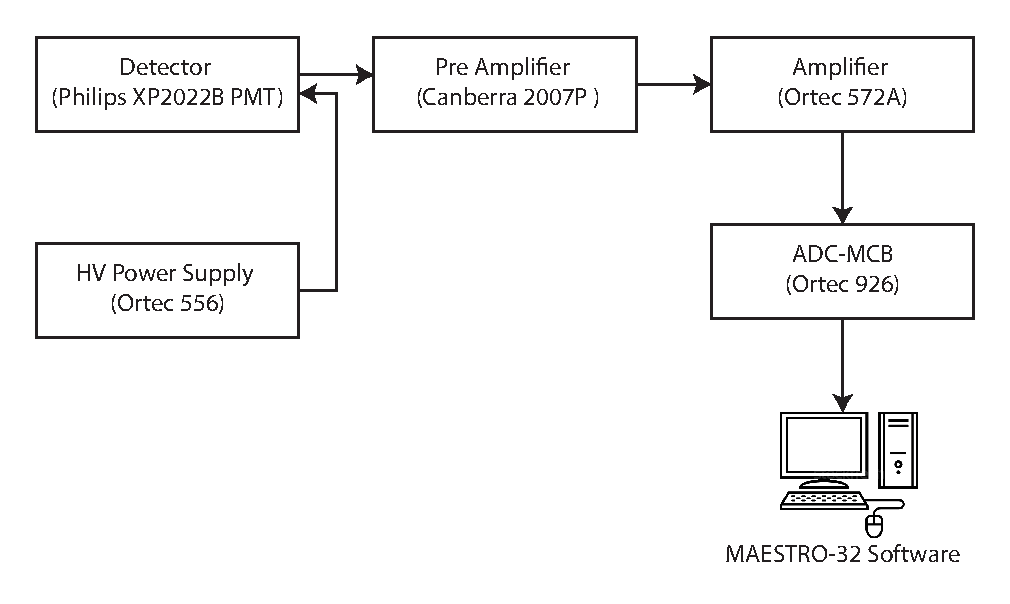
\includegraphics[width=\figurewidth]{ElectronicsSpectra}
	\caption{Pulse height measurement electronics}
	\label{fig:ElectronicsSpectra}
\end{figure}
A 100 $\mu$Ci \iso{Co}{60} source was used to measure the gamma energy deposition of the films, while a moderated \iso{Cf}{252} source was used for the neutrons.
The \iso{Cf}{252} irridiator contains two detector wells; a lead well and a cadmium well.
The lead well measures the response of neutron of all energies, while the cadmium well measures the responses of fast neutrons (Figure ~\ref{fig:SimPbCdSpectra}).
The two responses are then subtracted.
\begin{figure}
	\centering
	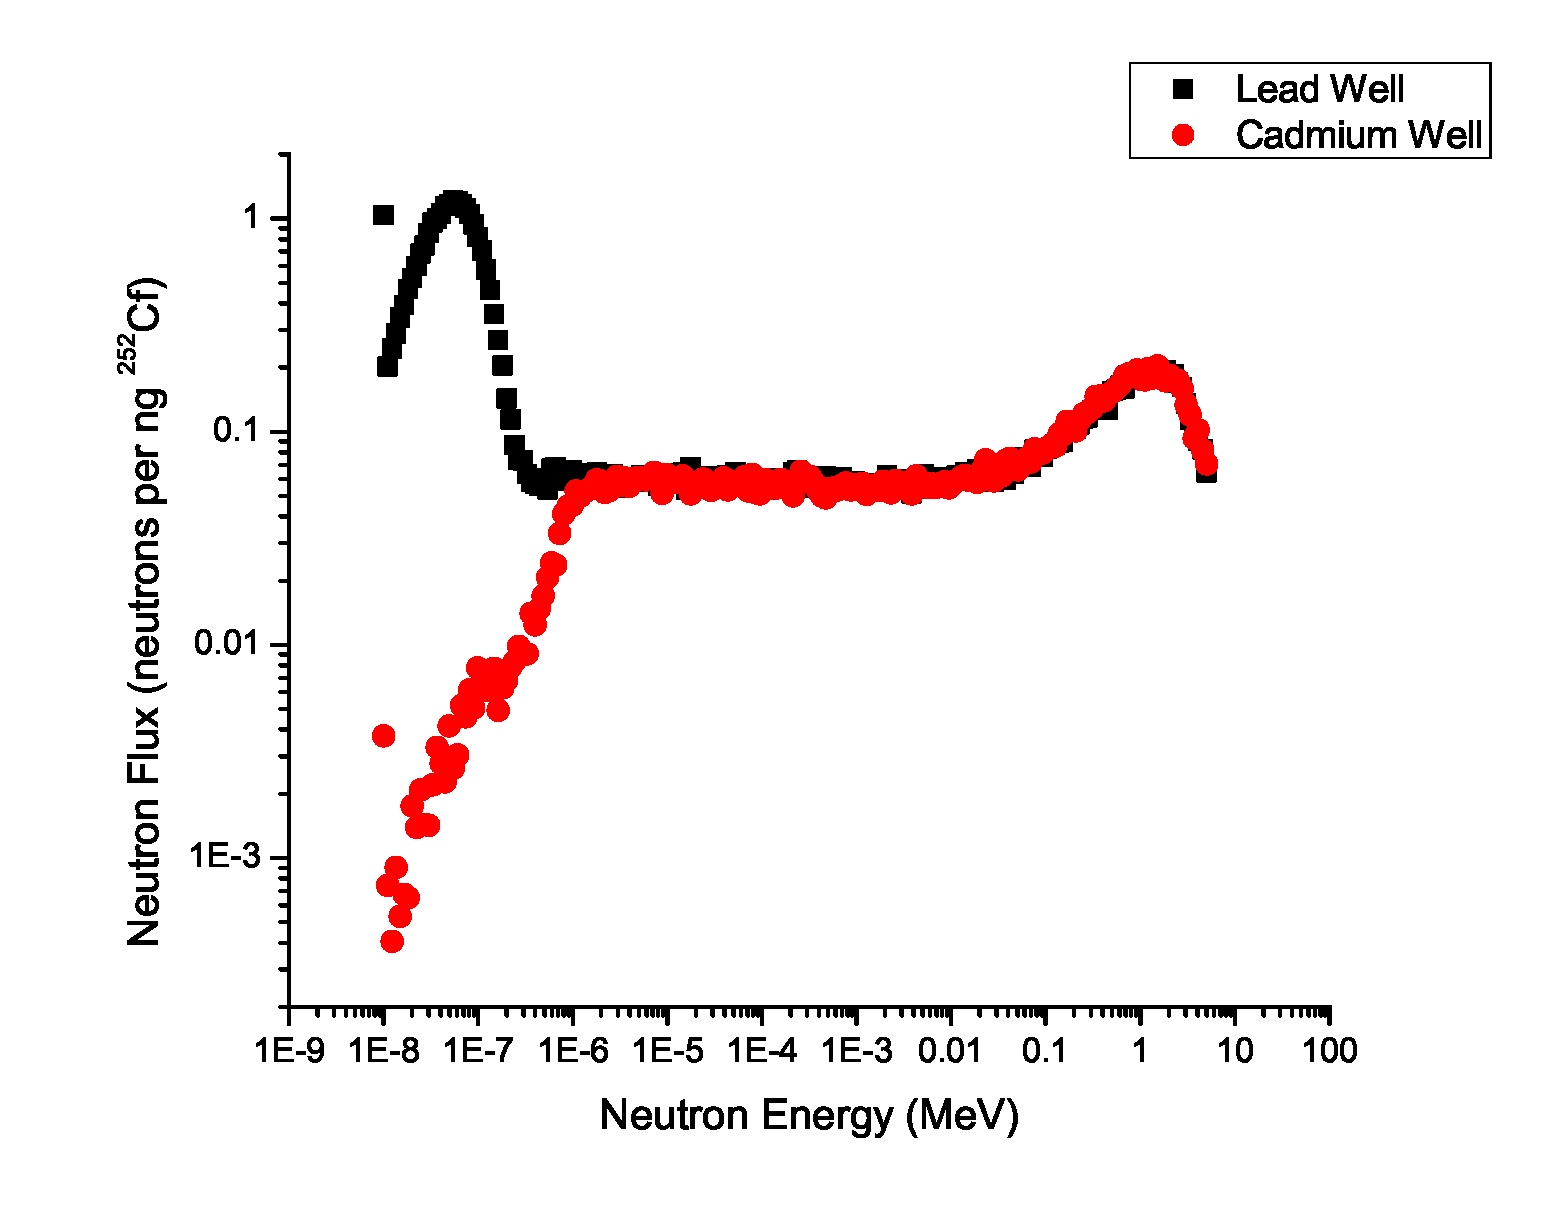
\includegraphics[width=\figurewidth]{Graph19N}
	\caption{Simulated Lead and Cadmium Well Spectra. The difference between the two spectra is the thermal neutron response and is what is measured.}
	\label{fig:SimPbCdSpectra}
\end{figure}
%%%%%%%%%%%%%%%%%%%%%%%%%%%%%%%%%%%%%%%%%%%%%%%%%%%%%%%%%%%%%%%%%%%%%%%%%%%
%                                                                         %
%                     RESULTS and ANALYSIS                                %
%                                                                         %
%%%%%%%%%%%%%%%%%%%%%%%%%%%%%%%%%%%%%%%%%%%%%%%%%%%%%%%%%%%%%%%%%%%%%%%%%%%
\section{Results}
It is well established that the pulse height of a radiation event is proportional to the energy deposition of the event\cite{birks_scintillations_1951}.
Thus, the validity of the GEANT4 simulation can be determined by comparing the spectra shapes of measured spectra to simulated energy deposition.
This was quantivied by computing the average energy deposition and the average pulse height.
With the average energy deposition on the left axis and the average light yield (pulse height) on the right axis, it is possible to compare the measurement and the simulation and agreement is observed, as in shown in Figure ~\ref{fig:EDepLightYield}. 
\begin{figure*}[!ht]
	\centering
	\begin{subfigure}[b]{\figurewidth}
    		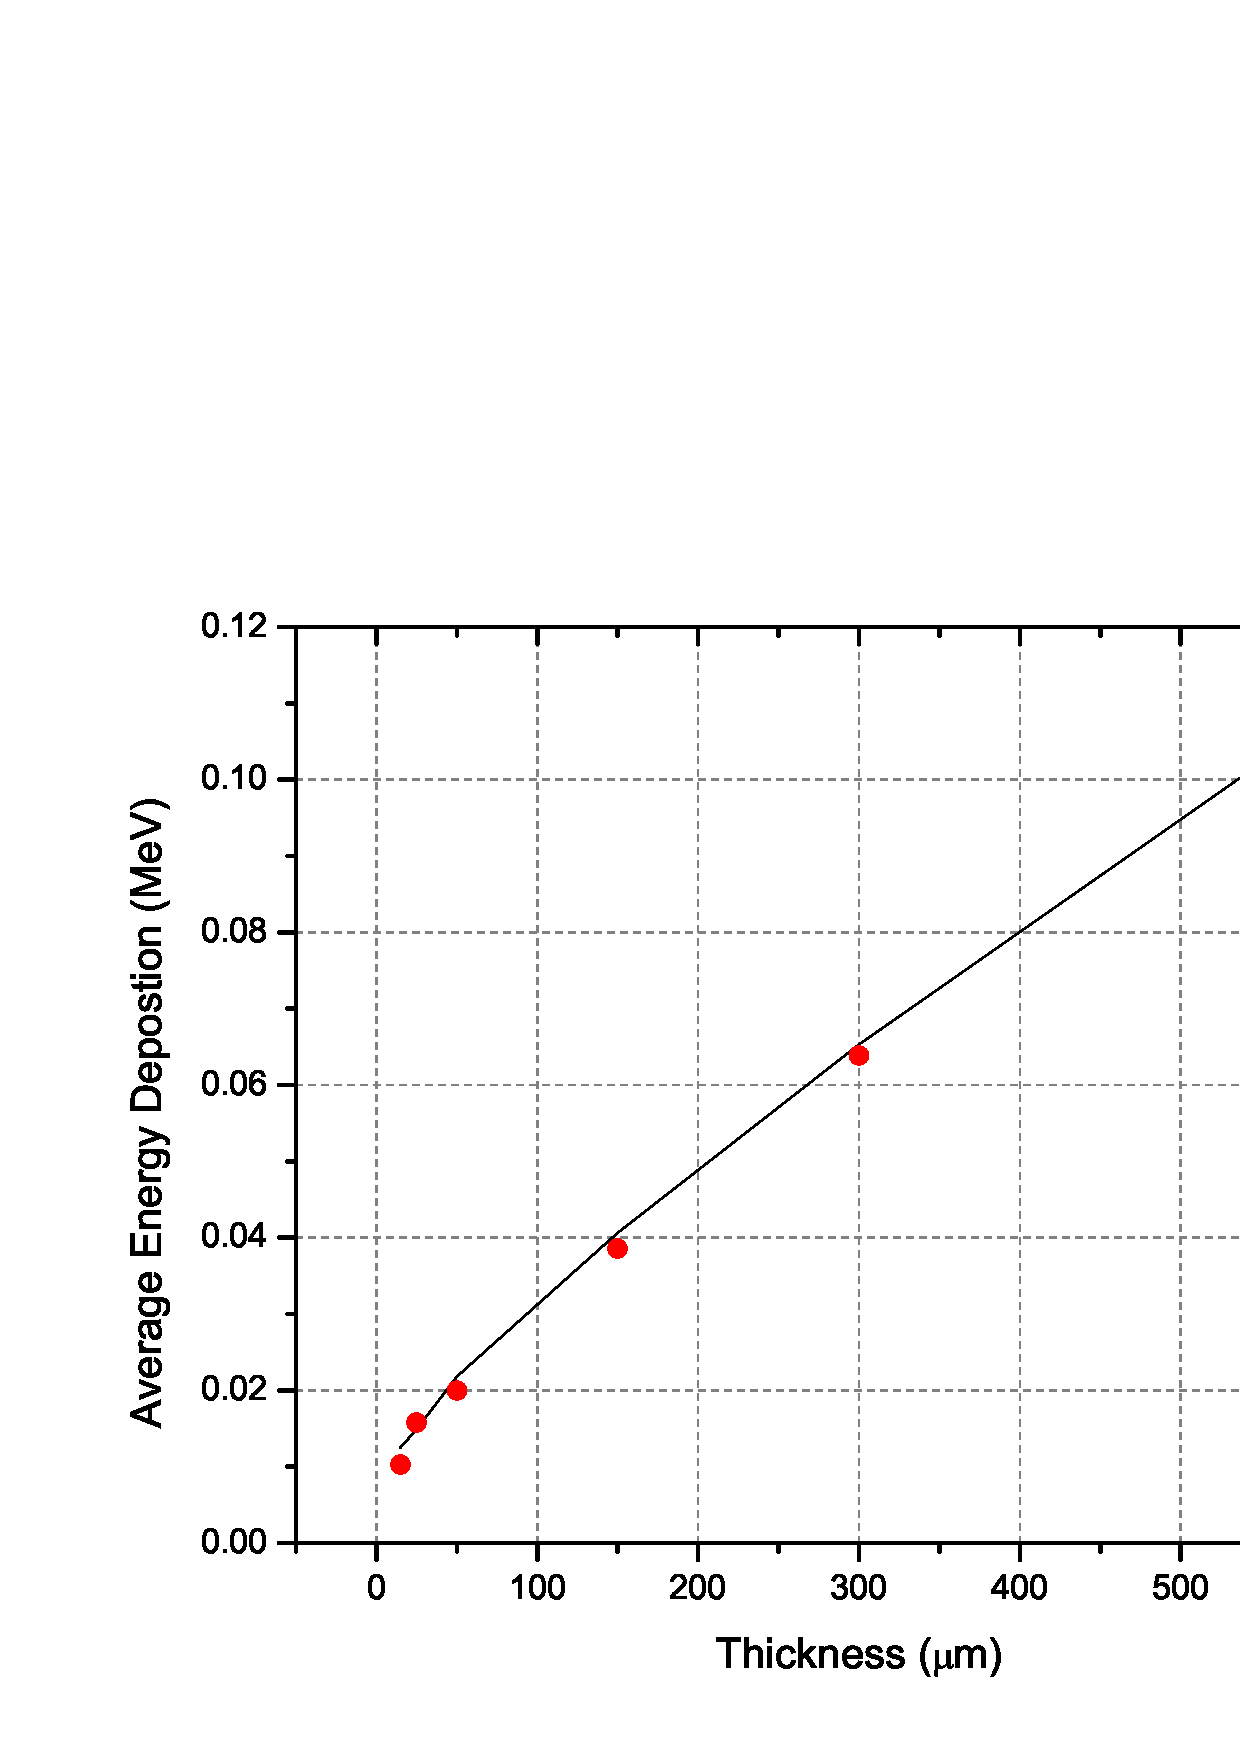
\includegraphics[width=\textwidth]{G4EDep_LightYield_Co60}
		\caption{Gamma (\iso{Co}{60})}
	\end{subfigure}%
	~
	\begin{subfigure}[b]{\figurewidth}
    		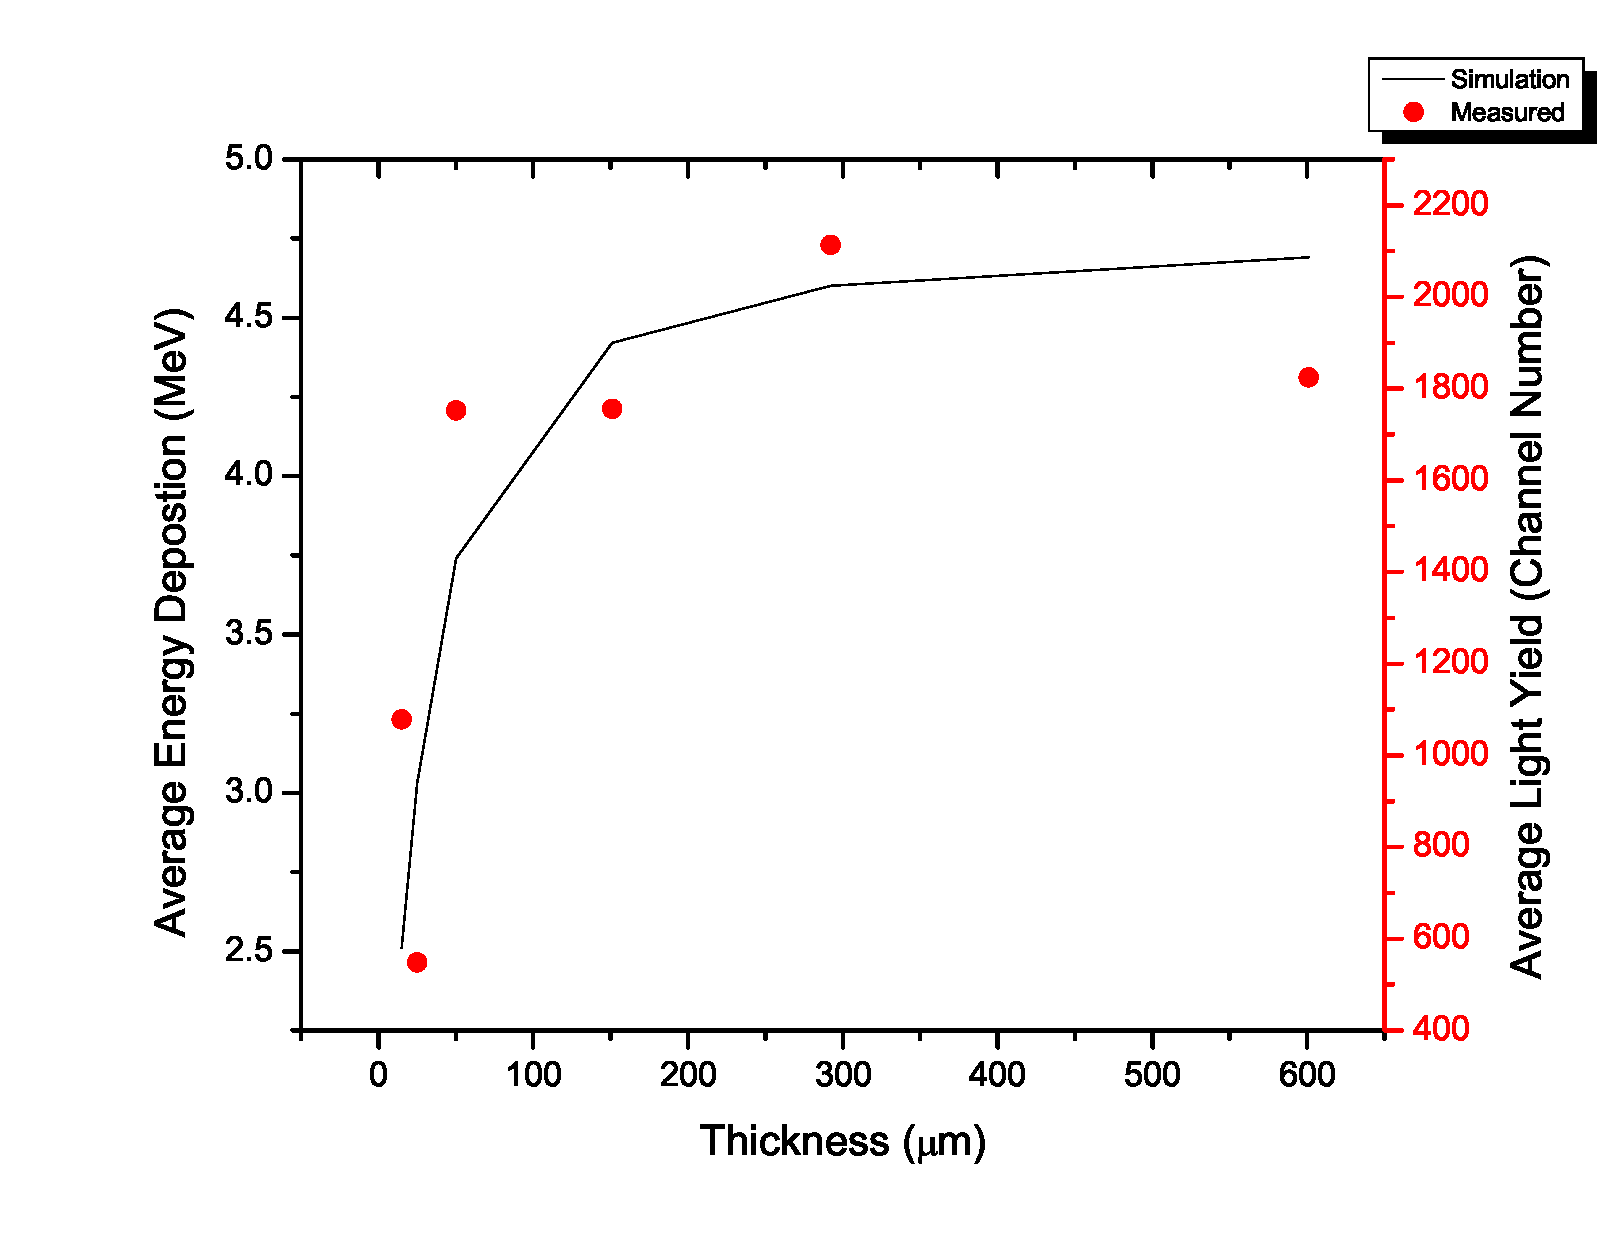
\includegraphics[width=\textwidth]{G4EDep_LightYield_Neutron}
		\caption{Neutrons}
	\end{subfigure}%
	\caption{Average Energy Deposition and Measured Light Yield}
	\label{fig:EDepLightYield}
\end{figure*}
%%%%%%%%%%%%%%%%%%%%%%%%%%%%%%%%%%%%%%%%%%%%%%%%%%%%%%%%%%%%%%%%%%%%%%%%%%%
%                                                                         %
%                             CONCLUSIONS                                 %
%                                                                         %
%%%%%%%%%%%%%%%%%%%%%%%%%%%%%%%%%%%%%%%%%%%%%%%%%%%%%%%%%%%%%%%%%%%%%%%%%%%
\section{Conclusions and Future Work}
The energy deposition for neutrons and gammas was calculated in thin polymeric films of thickness from 15 \micron to 1 cm with the GEANT4 toolkit and compared to the measured spectra.
The average energy deposited was computed for each thickness and and normalized by the incident energy for gammas or the Q-value of the reaction for neutrons, and is presented in Table ~\ref{tab:FractionEDep}, while the simulated energy deposition is shown in Figure ~\ref{fig:SimEDep}.
\begin{table}[!htb]
    \caption{Fractional Energy Deposition for Various Thickness}
	\centering
	\begin{tabular}{c | c c}
	Thickness & Gamma Fraction & Neutron Fraction \\
	\hline
	\hline
	15 \micron & 0.010 & 0.531 \\
	25 \micron & 0.013 & 0.634 \\
	50 \micron & 0.017 & 0.782 \\
	150 \micron & 0.032 & 0.927 \\
	300 \micron & 0.052 & 0.964 \\
	600 \micron & 0.087 & 0.982 \\
	1 mm & 0.130 & 0.989 \\
	1 cm & 0.425 & 0.998 \\
	\hline
	\end{tabular}
    \label{tab:FractionEDep}
\end{table}
\begin{figure*}[h]
	\centering
	\begin{subfigure}[b]{\figurewidth}
    		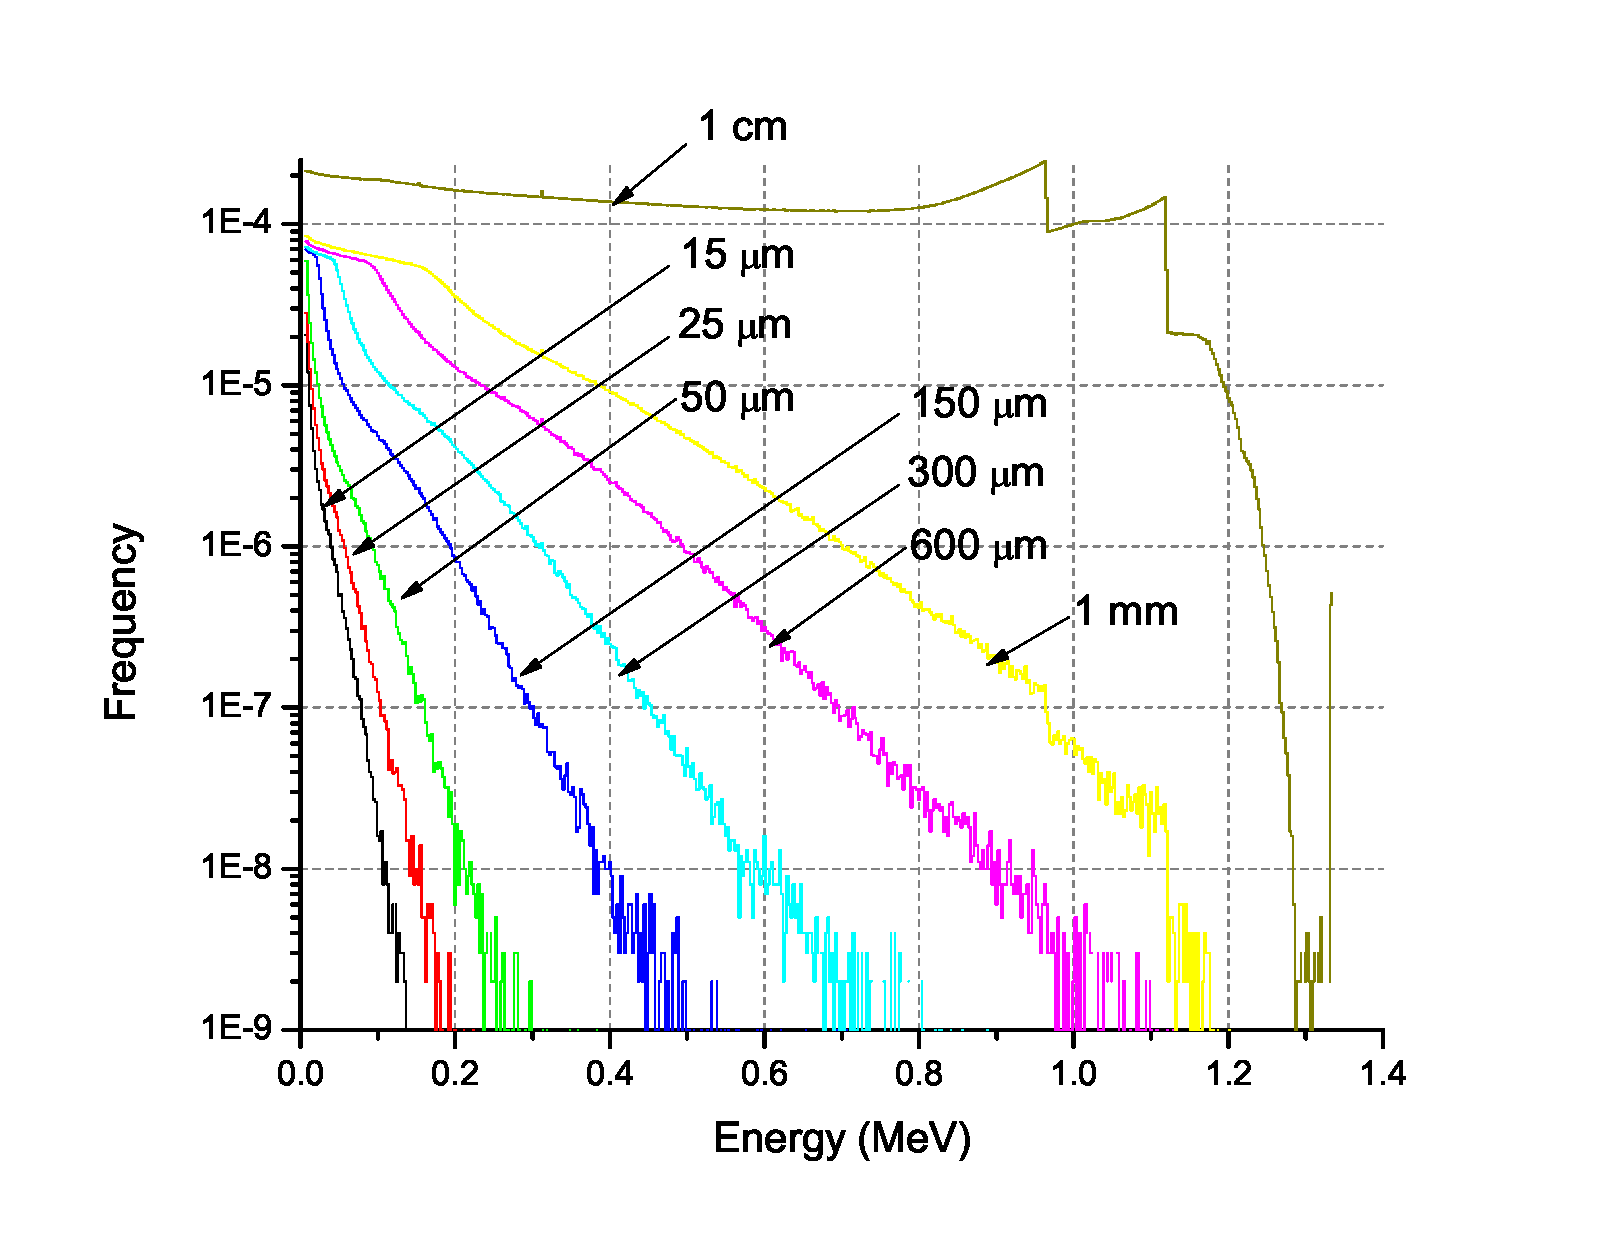
\includegraphics[width=\textwidth]{PS_EDepSim_Co60}
		\caption{Gamma (\iso{Co}{60})}
	\end{subfigure}%
	~
	\begin{subfigure}[b]{\figurewidth}
    		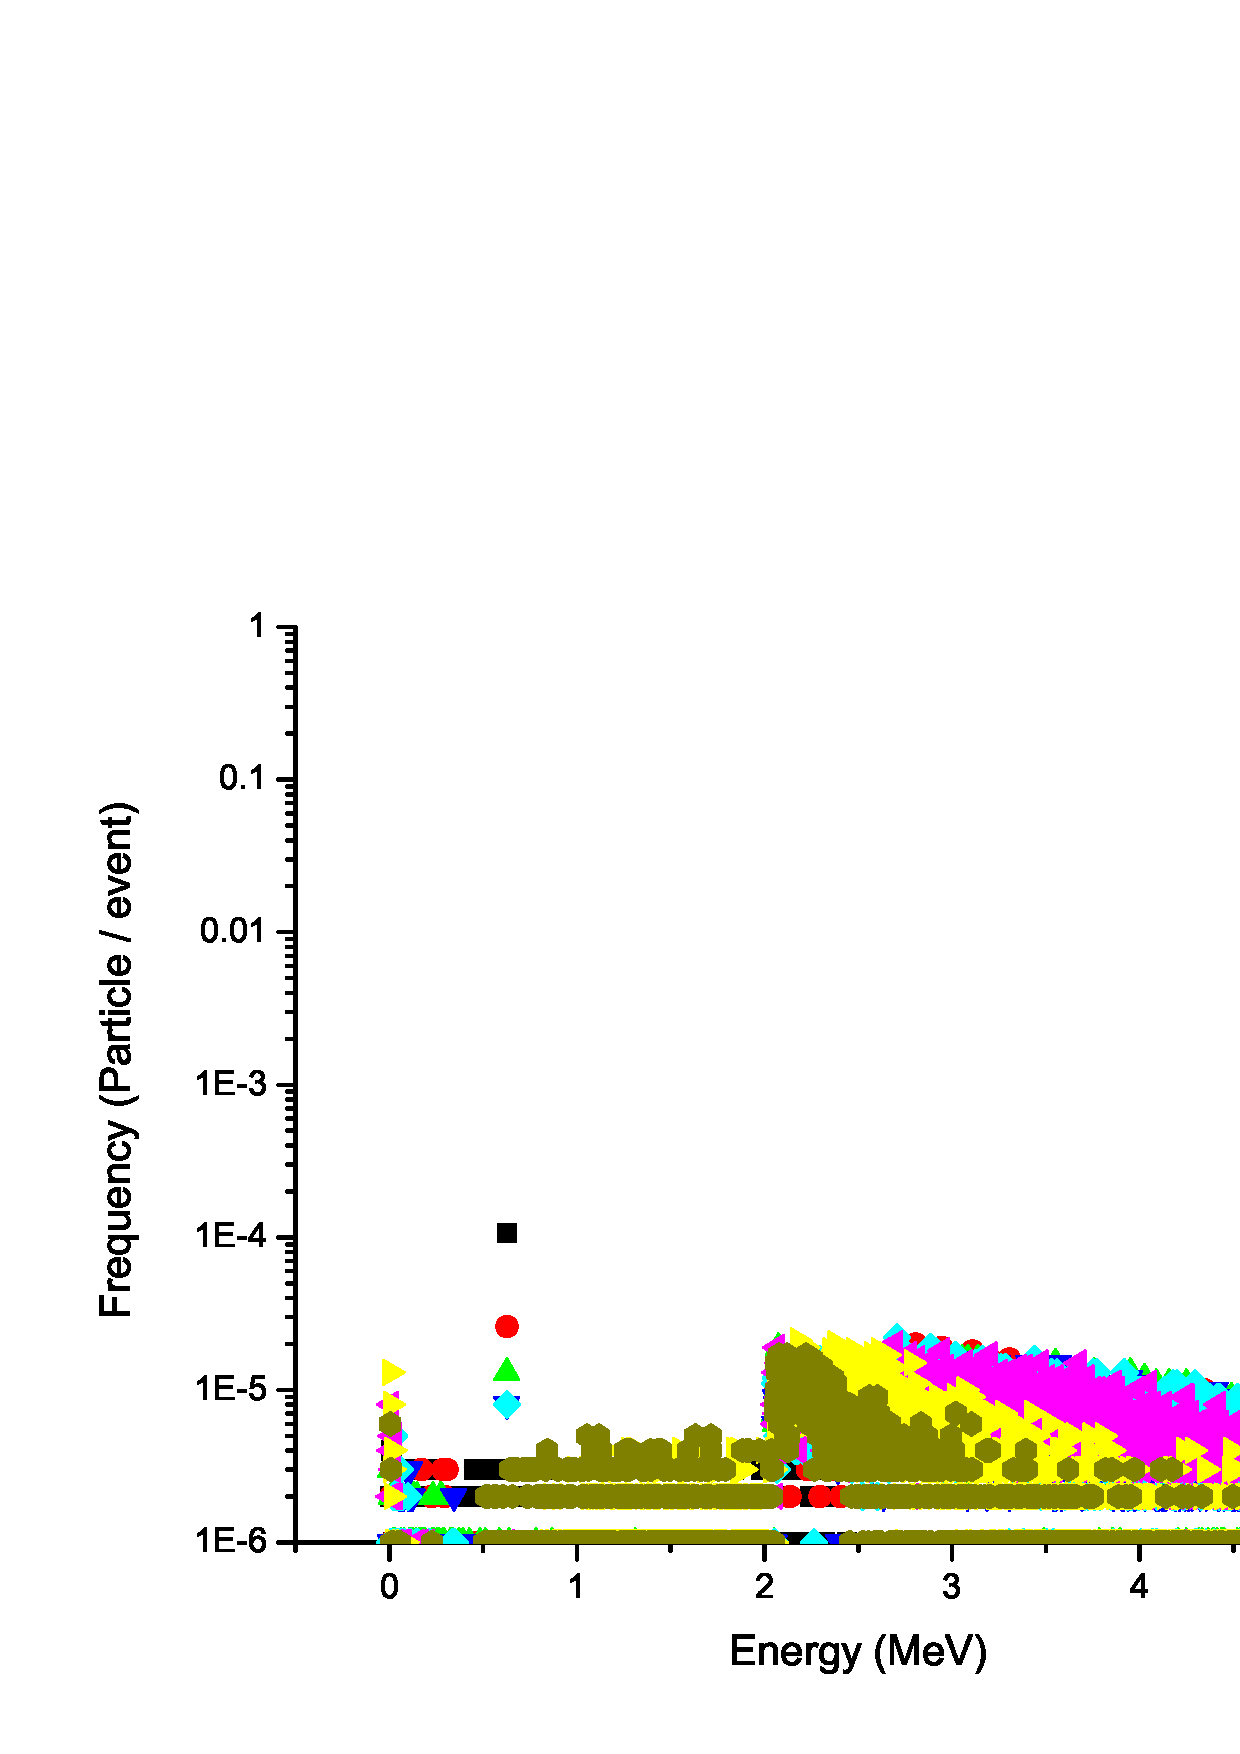
\includegraphics[width=\textwidth]{PS_EDepSim_Neutron}
		\caption{Neutrons}
	\end{subfigure}%
	\caption{Simulated Energy Deposition}
	\label{fig:SimEDep}
\end{figure*}
Future work will be focused on utilizing the GEANT4 toolkit to explore the energy deposition mechanisms in thin films, focusing on secondary electrons and their ranges. 
%%%%%%%%%%%%%%%%%%%%%%%%%%%%%%%%%%%%%%%%%%%%%%%%%%%%%%%%%%%%%%%%%%%%%%%%%%%%%%%%
\section{Acknowledgments}
This works was supported by the Domestic Nuclear Detection Office (DNDO) through award 003387891.
Any opinions, findings, and conclusions or recommendations expressed in this material are those of the authors and do necessarily reflect the views of DNDO.
%%%%%%%%%%%%%%%%%%%%%%%%%%%%%%%%%%%%%%%%%%%%%%%%%%%%%%%%%%%%%%%%%%%%%%%%%%%%%%%%
\bibliographystyle{ieeetr}
\bibliography{ANSBib}


\end{document}

